%%%%%%
% $Beschreibung: Vor der Montage erledigen $
% $Autor: Theilmann $
% $Datum: 11.06.2024 $
% $Version: 1 $
% $Pfad: SchrittmotorArduino\DemonstratorSchrittmotor\Assembly\VorMontage.tex $
%
%%%%%%
\chapter{Vor der Montage}
In diesem Kapitel werden die Vorarbeiten für die Montage erläutert. Es werden alle Bauteile, elektrischen Komponenten, benötigten Werkzeuge, das Vorbereiten der Leitungen und das Einsetzen der Einpressmuttern beschrieben.

\section{Bauteile}
In Abbildung \ref{Bauteile} werden alle Bauteile gezeigt in der Tabelle \ref{BauTab} benannt.

\begin{figure}[H]
	\begin{center}
		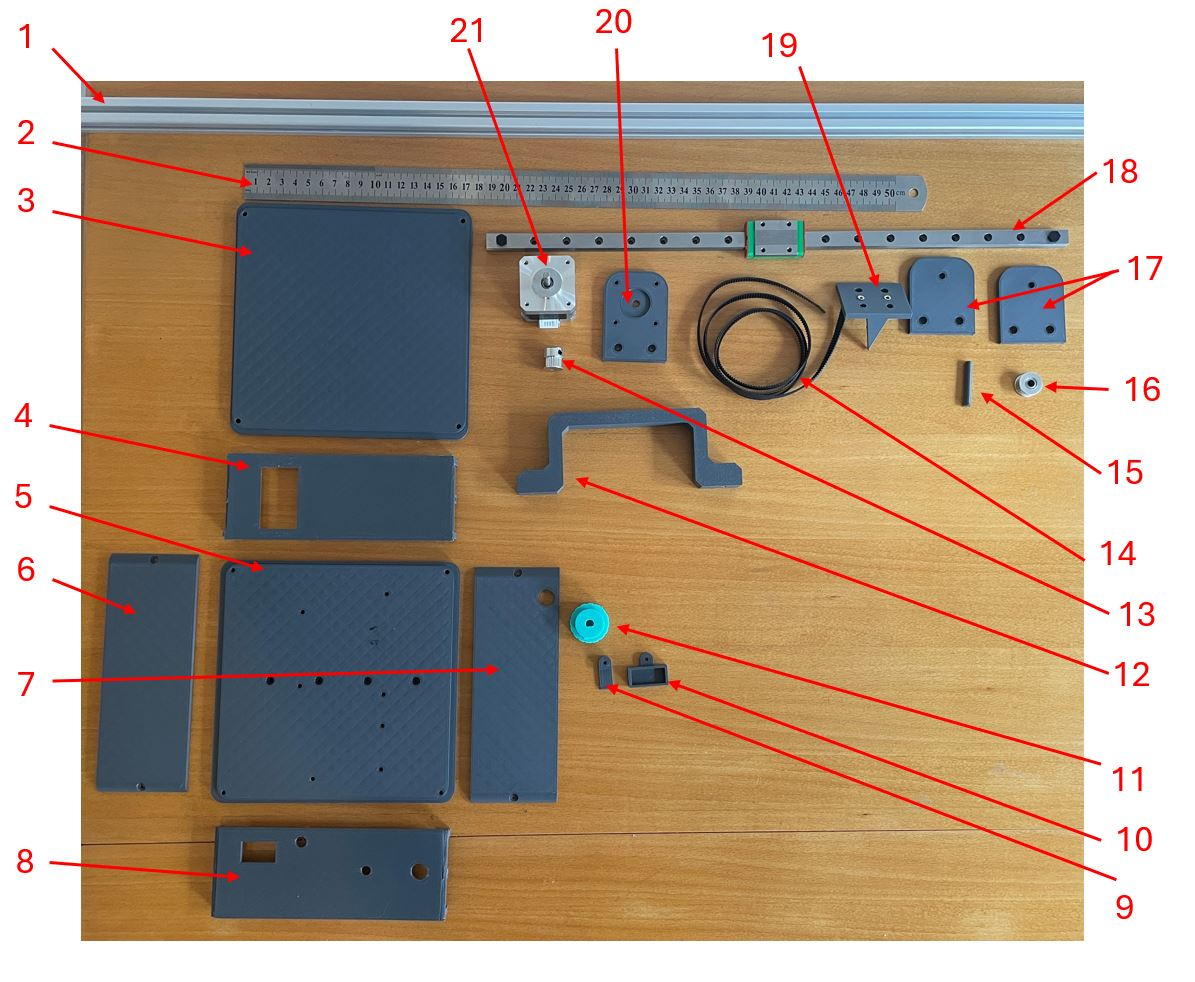
\includegraphics[width=\textwidth]{Images/BauTeile.jpg}
		\caption{Bauteile} \label{Bauteile}
	\end{center}
\end{figure}

\begin{figure}[htp]
	\begin{center}
		\fontsize{8}{10}\selectfont
		\begin{tabularx}{\textwidth}{|p{0.4cm}|X|X|X|X|X|} 
			\hline 
			\textbf{Pos.} &  \textbf{Benennung} \\ \hline
			1 & AluProfil   \\ \hline
			2 & Linieal   \\ \hline
			3 & Deckelplatte   \\ \hline
			4 & Hinterplatte   \\ \hline
			5 & Bodenplatte   \\ \hline
			6 & Seitenplatte Links \\ \hline
			7 & Seitenplatte Rechts  \\ \hline
			8 & Vorderplatte  \\ \hline
			9 & Klipp  \\ \hline
			10 & Halter für AMS  \\ \hline
			11 & Drehknopf  \\ \hline
			12 & Transportgriff  \\ \hline
			13 & Riemenantriebsscheibe  \\ \hline
			14 & Riemen  \\ \hline
			15 & Welle  \\ \hline
			16 & Riemenscheibe  \\ \hline
			17 & Halterung für die Welle  \\ \hline
			18 & Liniearführung  \\ \hline
			19 & Anzeiger  \\ \hline
			20 & Halterung für den Motor  \\ \hline
			21 & Nema 17 Motor  \\ \hline		
				
		\end{tabularx}
		\captionof{table}{Bauteile}	\label{BauTab}
	\end{center}
\end{figure}


\section{Elektrische Komponenten}
In Abbildung \ref{Bauteile} werden alle elektrischen Komponenten gezeigt in der Tabelle \ref{ElekTab} benannt.

\begin{figure}[H]
	\begin{center}
		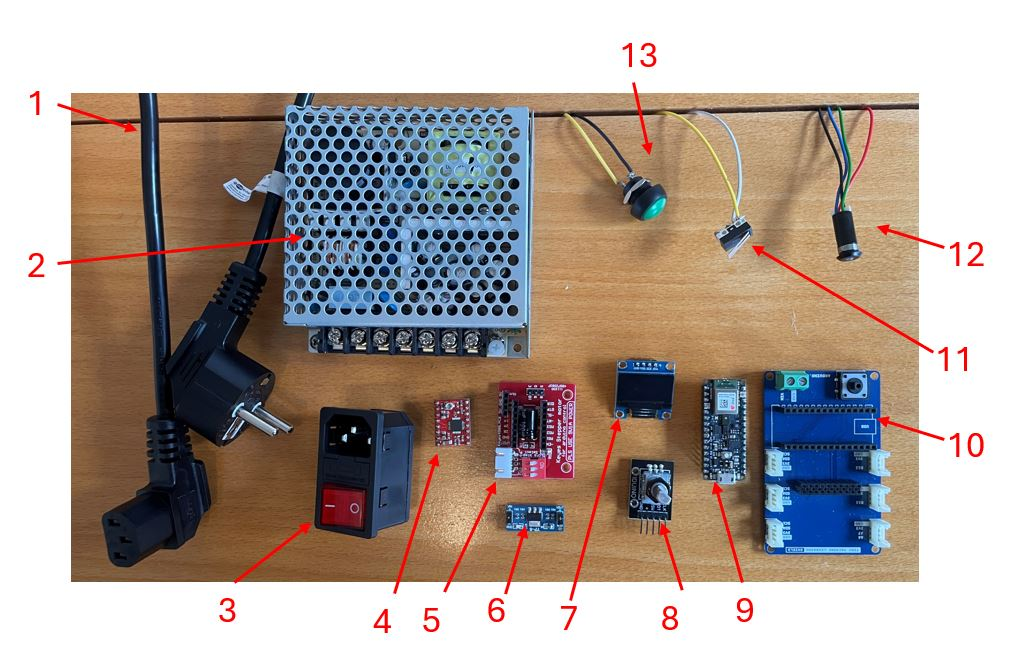
\includegraphics[width=\textwidth]{Images/ElekKomp.jpg}
		\caption{Elektrische Komponenten} \label{ElekKomb}
	\end{center}
\end{figure}

\begin{figure}[H]
	\begin{center}
		\fontsize{8}{10}\selectfont
		\begin{tabularx}{\textwidth}{|p{0.4cm}|X|X|X|X|X|} 
			\hline 
			\textbf{Pos.} &  \textbf{Benennung} \\ \hline
			1 & Netzkabel   \\ \hline
			2 & Schaltnetzteil   \\ \hline
			3 & Kaltgeräteanschluss   \\ \hline
			4 & Schrittmotorsteuerung A4988   \\ \hline
			5 & Entwicklerboard Schrittmotorsteuerung A4988   \\ \hline
			6 & Spannungswandler AMS1117 \\ \hline
			7 & OLED-Display  \\ \hline
			8 & Drehwinkel-Encoder  \\ \hline
			9 & Arduino Nano Sense BLE 33 Lite  \\ \hline
			10 & Arduino Tiny Maschnine Learning Shield (TMLS) \\ \hline
			11 & Micro-Schalter  \\ \hline
			12 & SMD-LED \\ \hline
			13 & Drucktaster  \\ \hline
					
		\end{tabularx}
		\captionof{table}{Elektrische Komponenten}	\label{ElekTab}
	\end{center}
\end{figure}

\section{Benötigtes Werkzeug}
In der Abbildung \ref{Benwerk} sind die benötigten Werkzeuge gezeigt und in der Tabelle \ref{WerkTab} erklärt. 

\begin{figure}[H]
	\begin{center}
		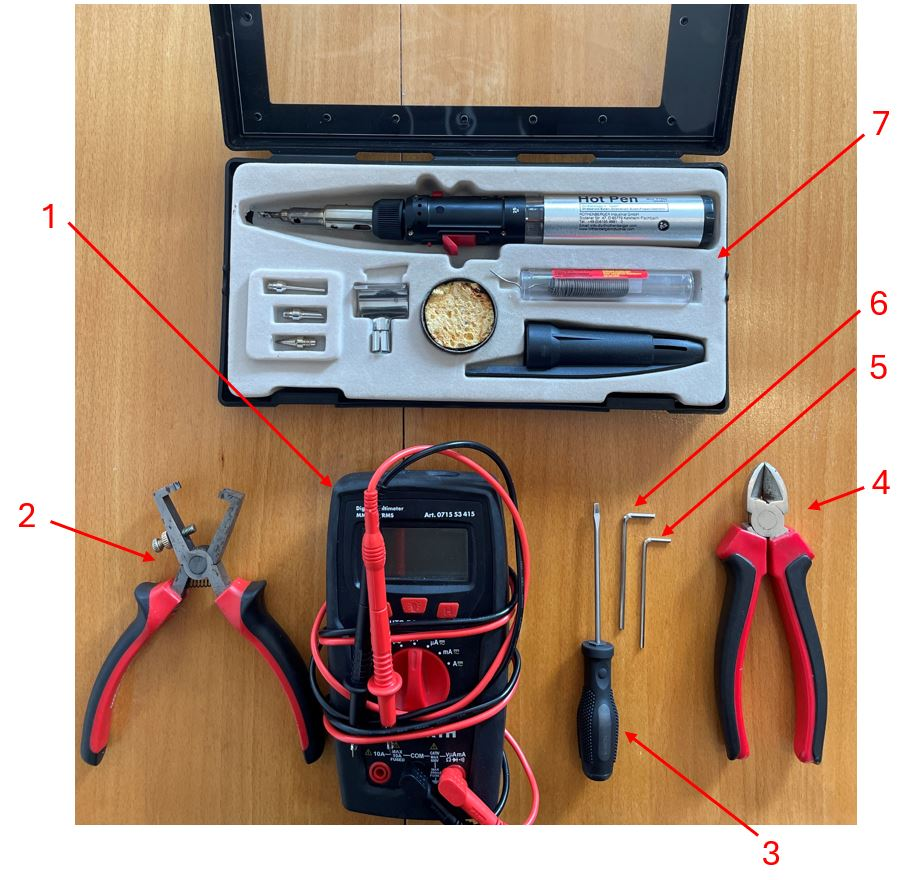
\includegraphics[width=\textwidth]{Images/BenWerk.jpg}
		\caption{Benötigtes Werkzeug} \label{Benwerk}
	\end{center}
\end{figure}

\begin{figure}[H]
	\begin{center}
		\fontsize{8}{10}\selectfont
		\begin{tabularx}{\textwidth}{|p{0.4cm}|p{3.4cm}|X|X|X|X|} 
			\hline 
			\textbf{Pos.} &  \textbf{Benennung} &  \textbf{Beschreibung}\\ \hline
			1 & Multimeter & Vielfachmessgerät zur Messung Elektrischer Größen z.B. Spannung, Strom und Widerstand  \\ \hline
			2 & Abisolierzange & Werkzeug zum Abisolieren elektrischer Leitungen  \\ \hline
			3 & Schraubendreher Schlitz 3 \ mm & Werkzeug zum hinein- oder herausschrauben von Schrauben \\ \hline
			4 & Seitenschneider & Werkzeug zum Trennen  \\ \hline
			5 & Innensechskantschlüssel 2 \ mm &  Werkzeug zum hinein- oder herausschrauben von Schrauben \\ \hline
			6 & Innensechskantschlüssel 2.5 \ mm &  Werkzeug zum hinein- oder herausschrauben von Schrauben \\ \hline
			7 & Lötkolben &  Gerät um Bauteile zu verlöten \\ \hline

		\end{tabularx}
		\captionof{table}{Benötigtes Werkzeug}	\label{WerkTab}
	\end{center}
\end{figure}

\section{Fertigung Bauteile}
Die aus der CAD-Software konstruierten STL-Dateien müssen per Slicer-Software an den jeweiligen 3D-Drucker angepasst werden. Daraufhin können die G-Codes an den 3D-Drucker exportiert und gedruckt werden. Die STL-Dateien finden Sie und dem Pfad: \emph{DemonstratorSchrittmotor \textbackslash Appendix \textbackslash Konstruktion \textbackslash STL}. Sollten Sie den Drucken von AnyCubic Modell Kobra Neo 2 benutzen, finden Sie die fertigen G-Codes unter dem Pfad: \emph{DemonstratorSchrittmotor \textbackslash Appendix \textbackslash Konstruktion \textbackslash GCodesAnyCubicKobra2Neo}
\section{Einsetzen der Einpressmuttern}
In den Bauteilen Vorderplatte, Hinterplatte und Anzeiger müssen die Einpressmuttern eingesetzt werden. In die \O 4 \ mm Bohrungen der Bauteile wird mit einem heißen Lötkolben die Einpressmutter eingesetzt bis diese bündig mit dem Bauteil sitzt. Dies ist Abbildung \ref{Einpress} zu sehen.

\begin{figure}[H]
	\begin{center}
		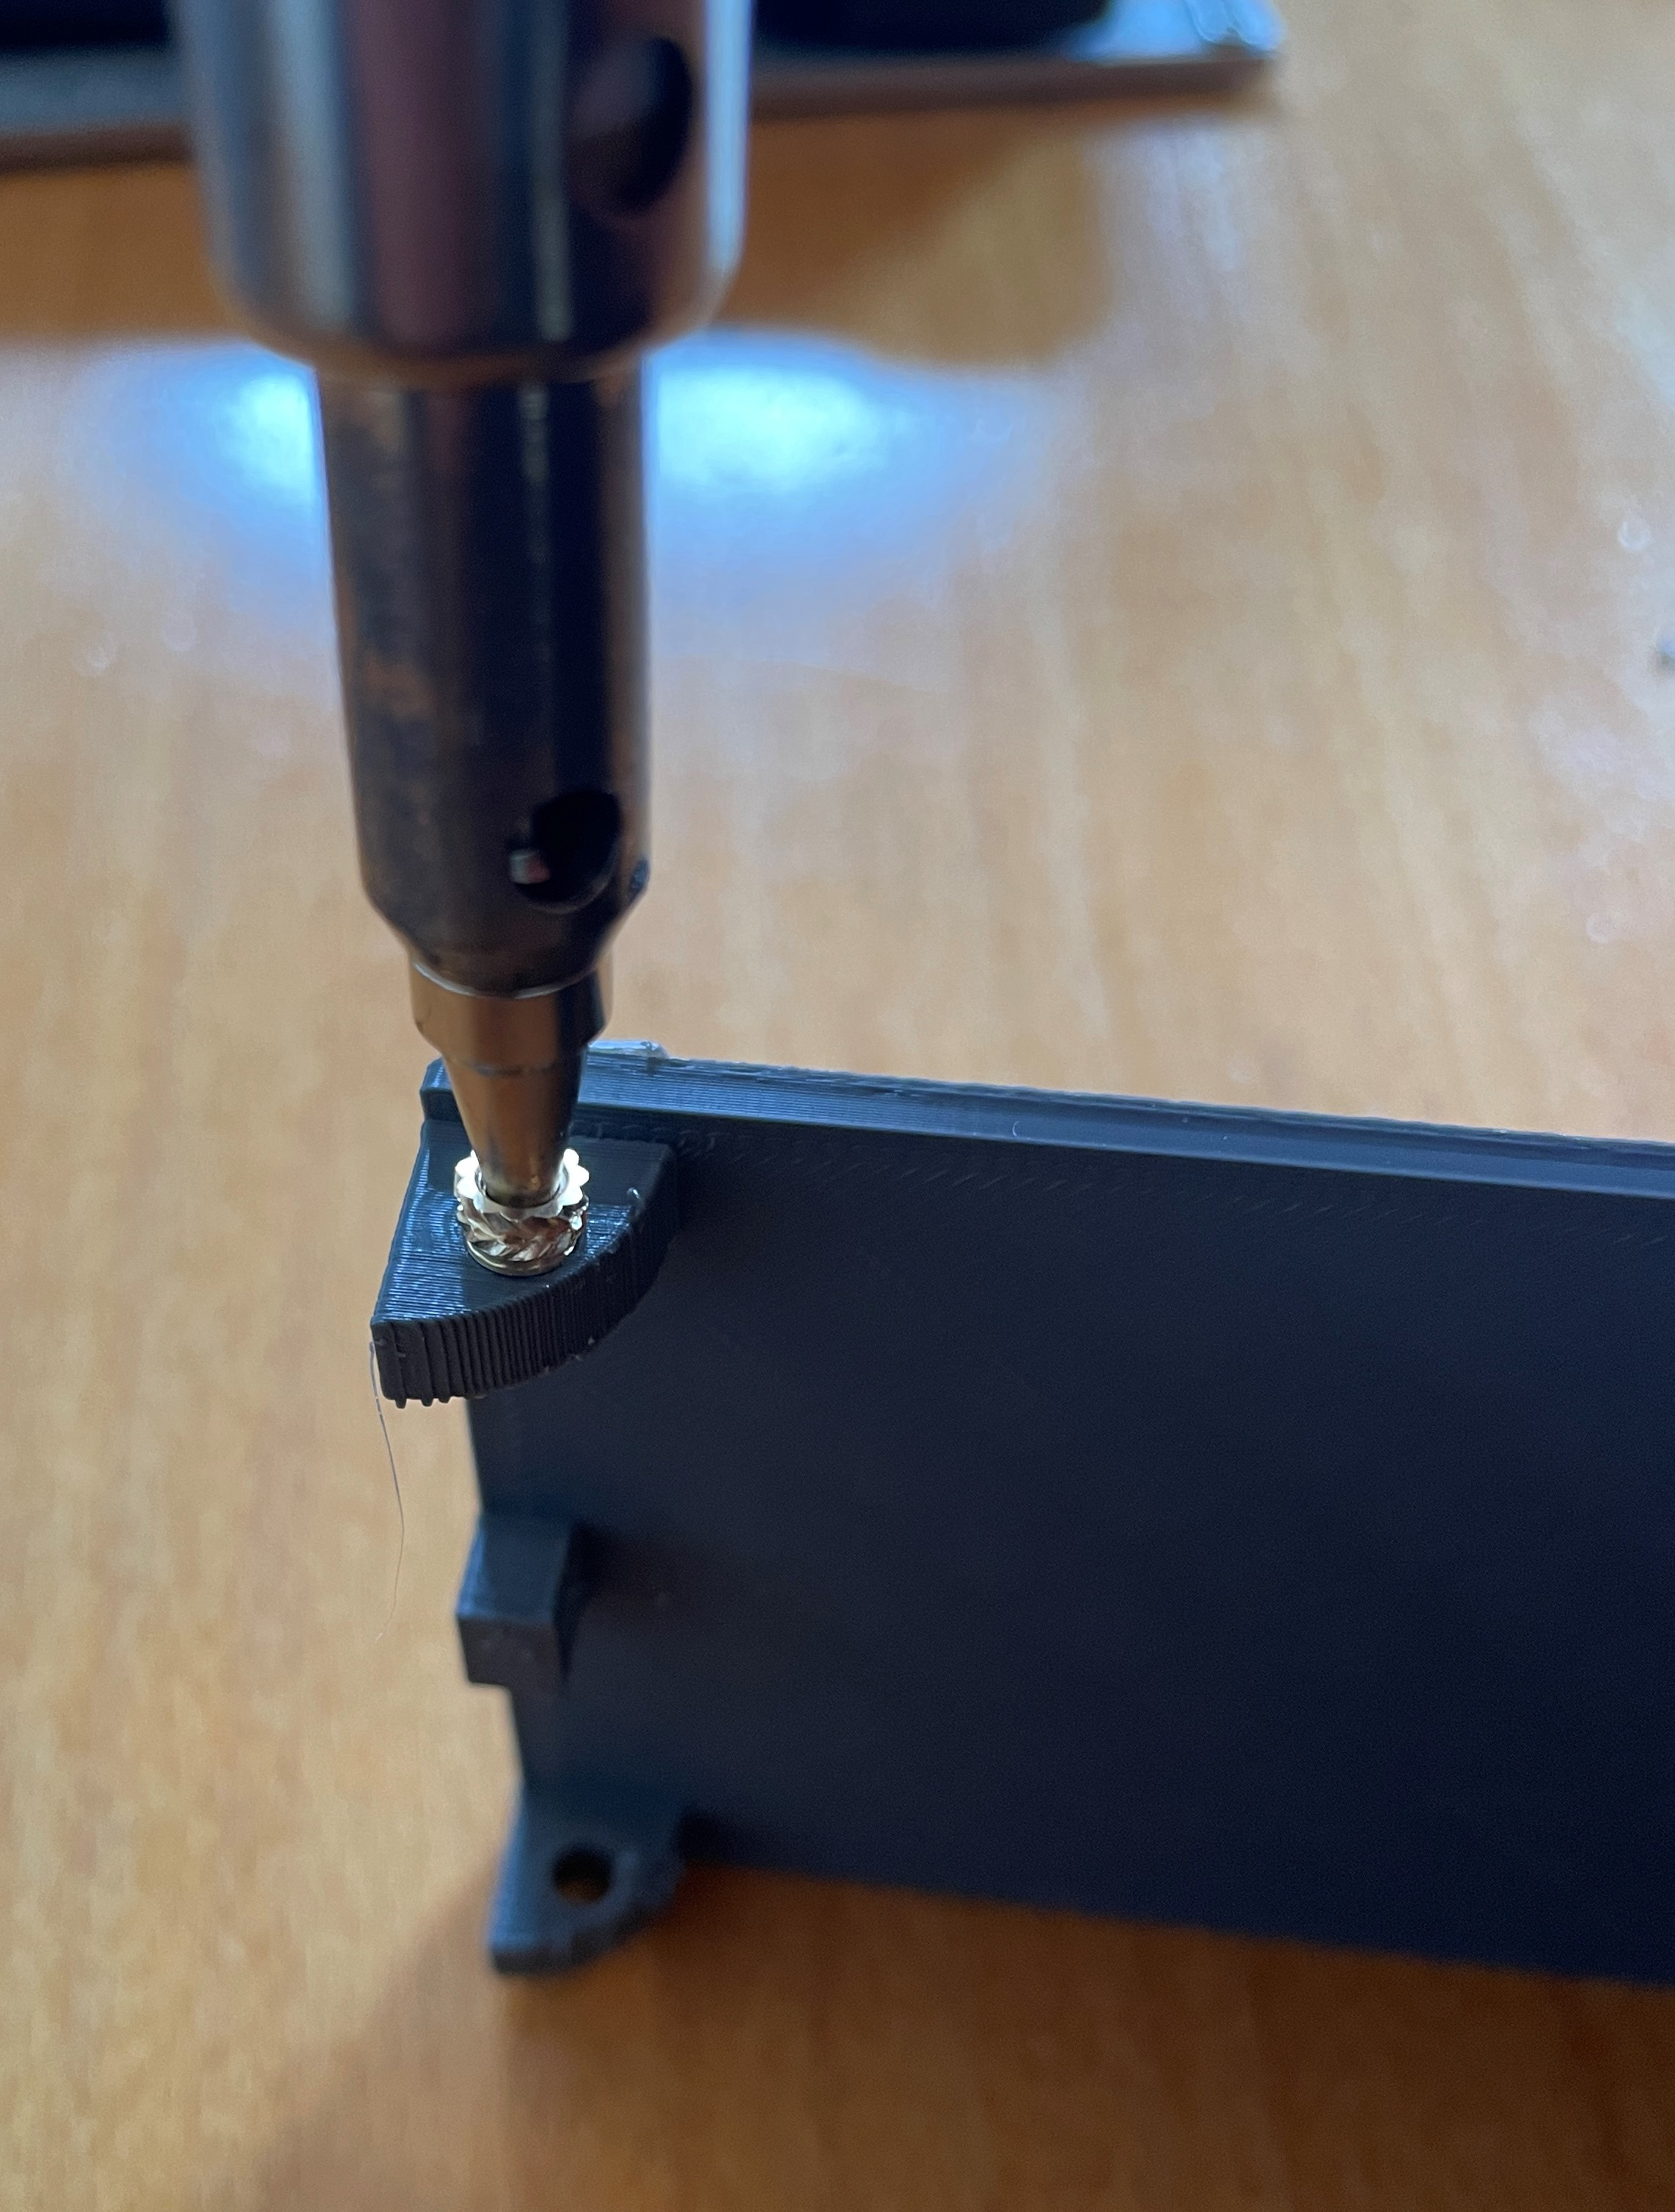
\includegraphics[width=\textwidth]{Images/Einpress.jpg}
		\caption{Einpressen der Einpressmuttern} \label{Einpress}
	\end{center}
\end{figure}

\section{Vorbereiten der elektrischen Leitungen}
Die elektrischen Leitungen werden vor der Montage vorbereitet, um ein einfacheres Montieren zu gewährleisten. Die benötigten Leitungen sind in Abbildung \ref{Leitungen} gezeigt und werden in Tabelle \ref{Leittab} mit den zugehörigen Leitungsenden aufgelistet. Des Weiteren werden die Verbindungsart, Länge und Benennung erwähnt.

\begin{figure}[H]
	\begin{center}
		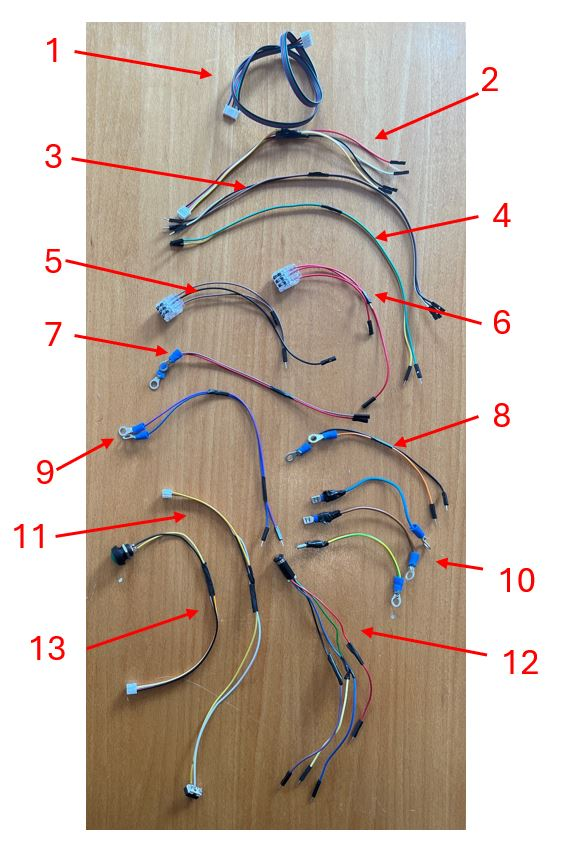
\includegraphics[width=\textwidth]{Images/Leitungen.jpg}
		\caption{Benötigte Leitungen} \label{Leitungen}
	\end{center}
\end{figure}

\begin{figure}[H]
	\begin{center}
		\fontsize{8}{10}\selectfont
		\begin{tabularx}{\textwidth}{|p{0.5cm}|p{0.5cm}|p{2.0cm}|p{2.0cm}|p{2.0cm}|X|p{0.7cm}|X|} 
			\hline 
			\textbf{Pos.} &  \textbf{Anz.} &  \textbf{Leitungsende 1} &  \textbf{Leitungsende 2} &  \textbf{Leitungsende 3} & \textbf{Verbind-ungsart} &  \textbf{Länge [mm]} &  \textbf{Benennung} \\ \hline
			1 & 1 & 6 Pin PH2.0 & 4 Pin XH2.54 & - & - & 250 & Entwicklerboard Schrittmotorsteuerung A4988 zu Nema 17 Motor \\ \hline
			2 & 1 & 4 Pin HY2.0 & 4 x Jumper Female & - & Löten & 230 & TMLS auf OLED-Display \\ \hline
			3 & 1 & 3 x Jumper Male & 3 x Jumper Female & - & - & 320 & TMLS auf Drehwinkel-Encoder \\ \hline
			4 & 1 & 2 x Jumper Male & 2 x Jumper Female & - & - & 320 & TMLS auf Entwicklerboard Schrittmotorsteuerung A4988 \\ \hline
			5 & 1 & 1 x Jumper Male & 1 x Jumper Female & 1 x Jumper Female & Hebelklemme & 190 & Masse Spannungswandler AMS117 auf Drehwinkel-Encoder und Entwicklerboard Schrittmotorsteuerung A4988 \\ \hline
			6 & 1 & 1 x Jumper Male & 1 x Jumper Female & 1 x Jumper Female & Hebelklemme & 190 & 3,3V Spannungswandler AMS117 auf Drehwinkel-Encoder und Entwicklerboard Schrittmotorsteuerung A4988 \\ \hline
			7 & 2 & 1 x Kabelschuh Ringform & 1 x Jumper Female &  - & Quetschen & 210 & 5V/Masse Schaltnetzteil auf Spannungswandler AMS117  \\ \hline
			8 & 2 & 1 x Kabelschuh Ringform & 1 x Jumper Male &  - & Quetschen & 250 & 12V/Masse Schaltnetzteil auf Entwicklerboard Schrittmotorsteuerung A4988  \\ \hline
			9 & 2 & 1 x Kabelschuh Ringform & 1 x Jumper Male &  - & Quetschen & 170 & 12V/Masse Schaltnetzteil auf TMLS  \\ \hline
			10 & 3 & 1 x Kabelschuh Ringform & 1 x Kabelschuh Flachsteckhülse & - & 1 x Quetschen & 125 & Kaltgerätean-schluss auf Schaltnetzteil  \\ \hline
			11 & 1 & 1 x Pin HY2.0 & 2 x Micro-Schalter & - & 1 x Löten & 285 & TMLS auf Micro-Schalter  \\ \hline
			12 & 1 & 4 x Jumper Male & SMD-LED & - & Löten & 225 & TMLS auf SMD-LED  \\ \hline
			13 & 1 & 1 x Pin HY2.0 & 2 x Druckknopf x & - & Löten & 230 & TMLS auf Druckknopf  \\ \hline
			
		\end{tabularx}
		\captionof{table}{Leitungen}	\label{Leittab}
	\end{center}
\end{figure}

\section{Schrauben und Muttern }
In der folgenden Tabelle \ref{Verbrauch} werden die benötigten Schrauben und Muttern aufgelistet

\begin{figure}[H]
	\begin{center}
		\fontsize{8}{10}\selectfont
		\begin{tabularx}{\textwidth}{|p{0.5cm}|p{0,8cm}|X|X|X|X|} 
			\hline 
			\textbf{Pos.} &  \textbf{Anzahl} &  \textbf{Beschreibung}\\ \hline
			1 & 17 & M3 Hammermutter T-Schlitz Nut 6  \\ \hline
			2 & 14 & Zylinderschrauben M3 6 \ mm Innensechskant DIN 912  \\ \hline
			3 & 16 & Zylinderschrauben M3 8 \ mm Innensechskant DIN 912 \\ \hline
			4 & 21 & Zylinderschrauben M3 10 \ mm Innensechskant DIN 912\\ \hline
			5 & 7  & Zylinderschrauben M3 14 \ mm Innensechskant DIN 912 \\ \hline
			6 & 7 & Sechskantmuttern M3 DIN 934  \\ \hline
			7 & 2 &  Senkschrauben M2.5 5 \ mm Kreuzschlitz Phillips  \\ \hline
			
		\end{tabularx}
		\captionof{table}{Benötigte Schrauben und Muttern}	\label{Verbrauch}
	\end{center}
\end{figure}

\section{Schaltplan}
Der Schaltplan zeigt die elektrische Verbindung der einzelnen Komponenten. Er ist in Abbildung \ref{Splan} dargestellt.

\begin{figure}[H]
	\begin{center}
		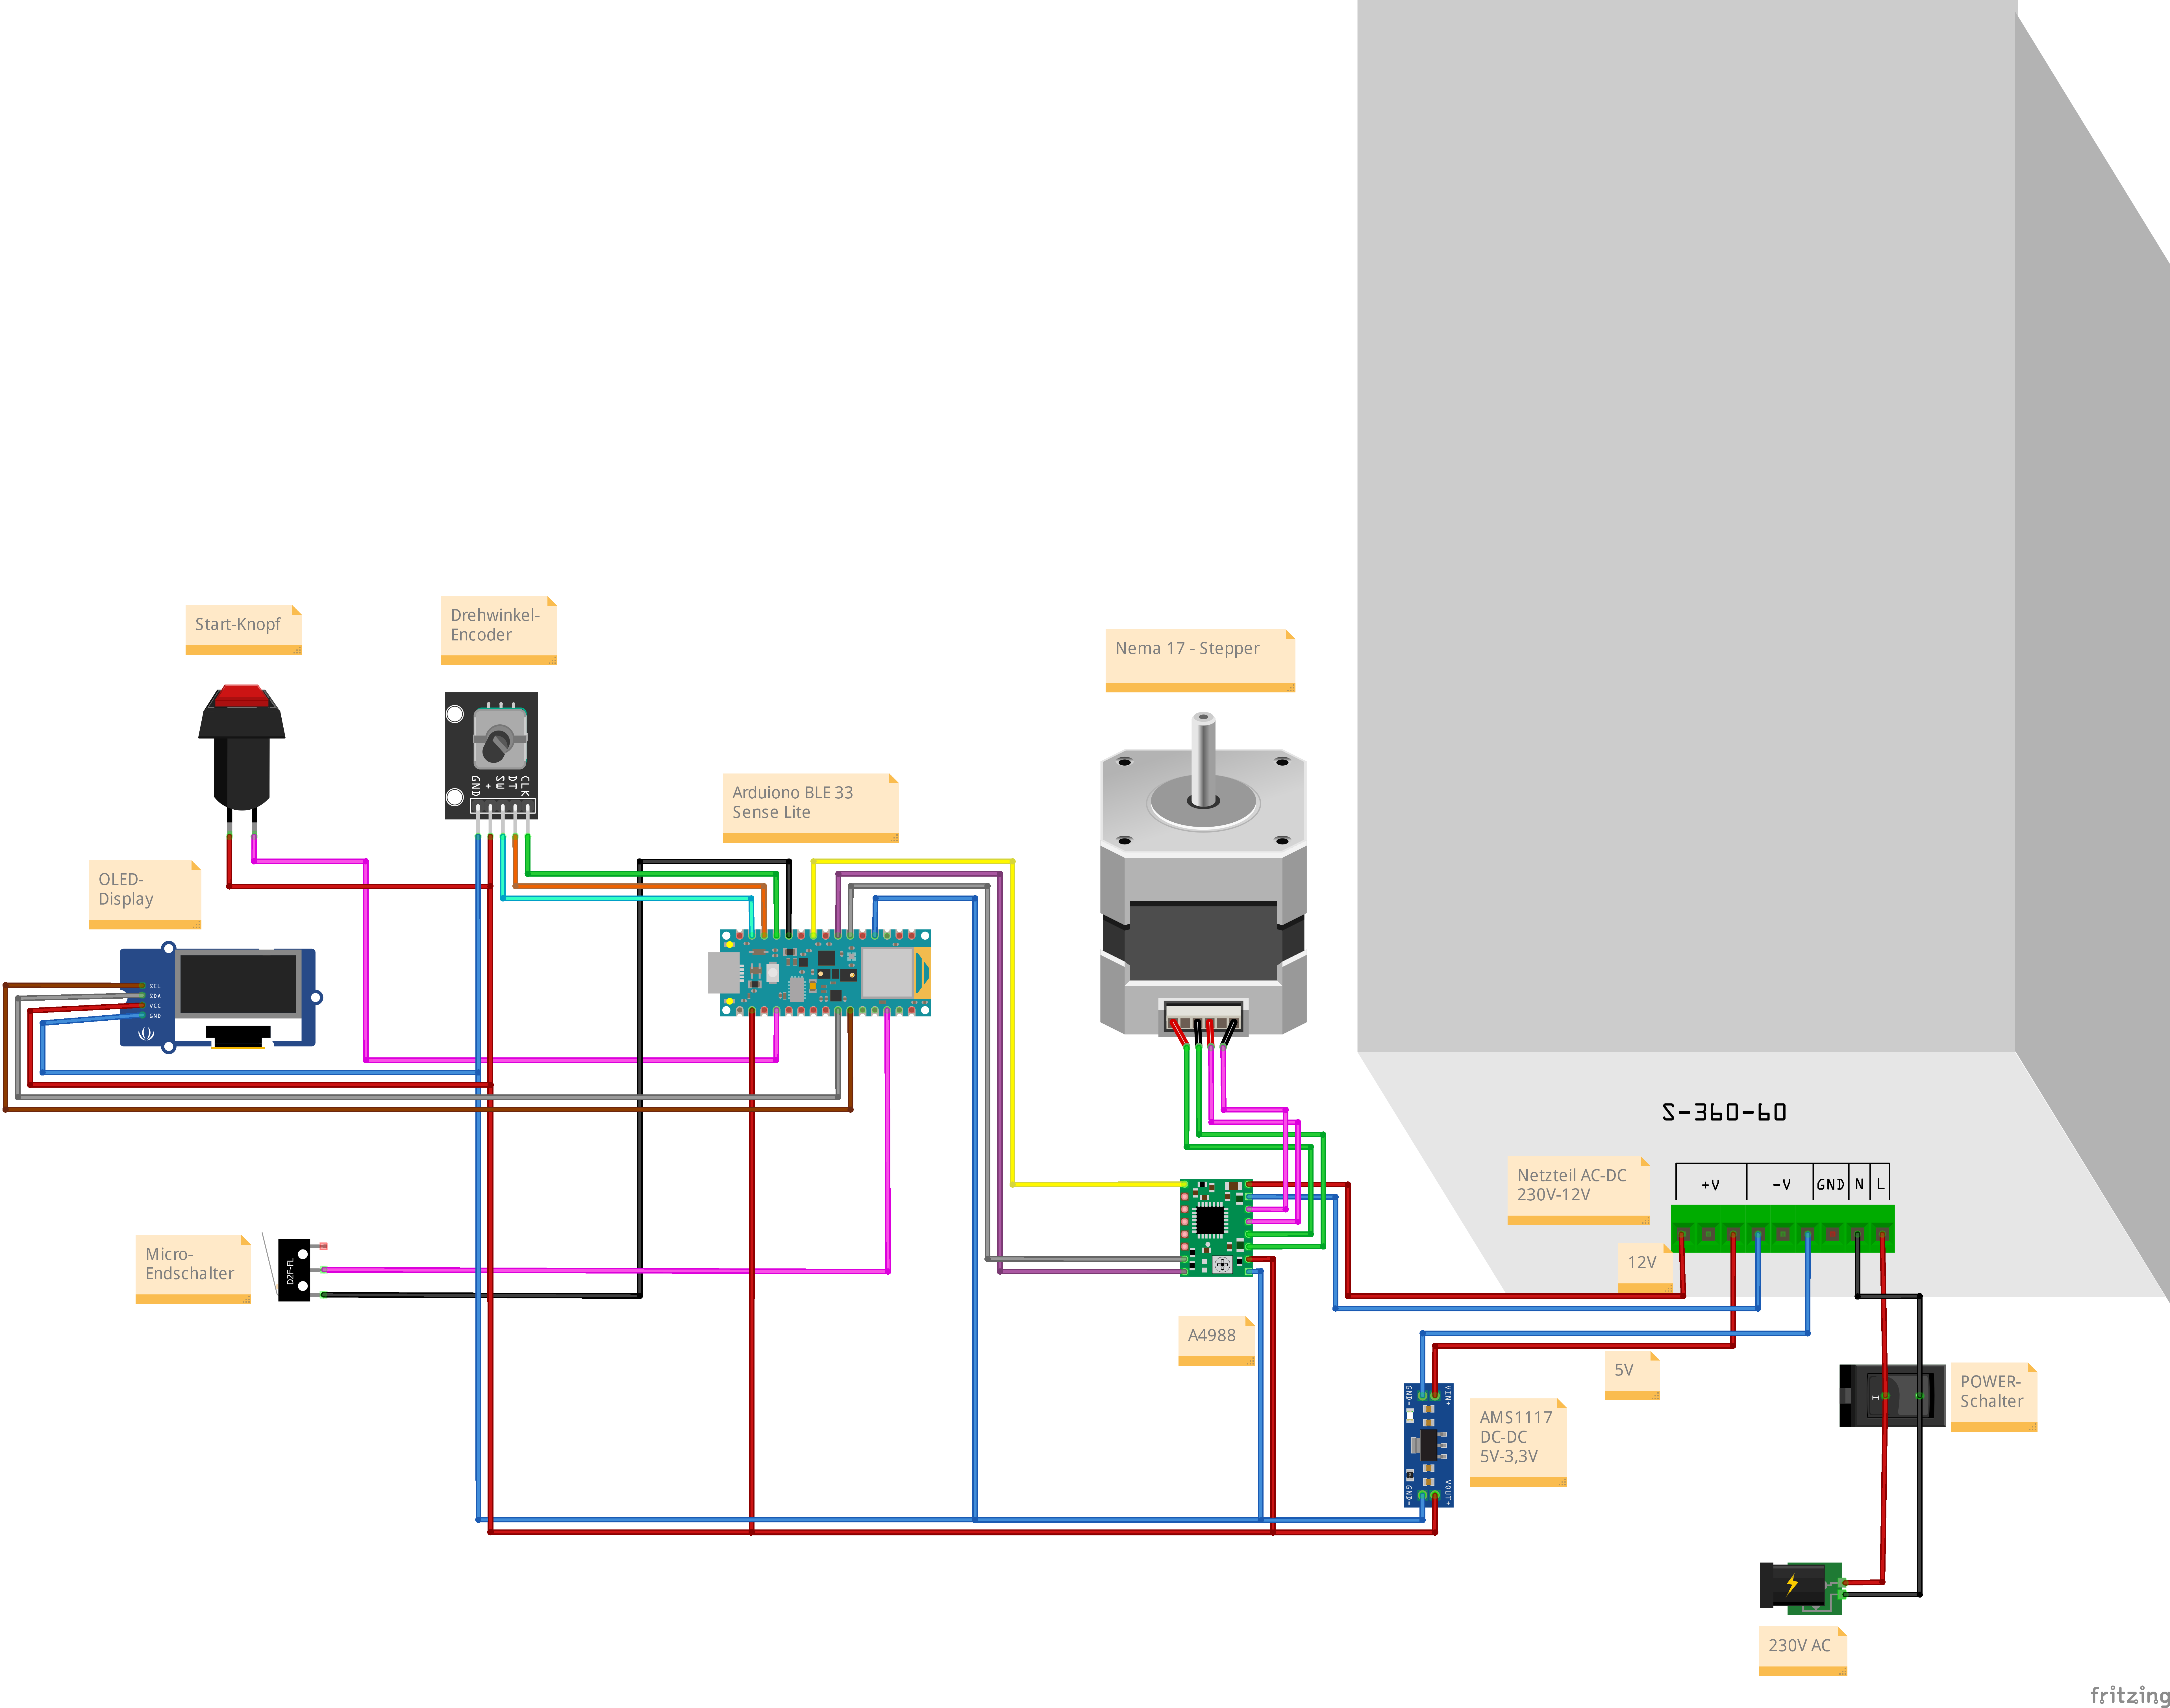
\includegraphics[width=\textwidth]{Images/Schaltplan1.png}
		\caption{Schaltplan} \label{Splan}
	\end{center}
\end{figure}

 